\chapter{Establishing the framework to reprogram a preadipocyte cell line into depot-specific adipocytes
}\label{chap:chapter 3}


%%%%%%%%%%%%%%%%%%%%%%%%%%%%%%%%%%%%%%%%%%%%%%%%%%%%%%%%%%%%%%%%%%%%%%%%%%%%%%%%
\section{Introduction}
%%%%%%%%%%%%%%%%%%%%%%%%%%%%%%%%%%%%%%%%%%%%%%%%%%%%%%%%%%%%%%%%%%%%%%%%%%%%%%%%

Adipose tissue is a dynamic endocrine organ that plays a central role in maintaining metabolic homeostasis. Adipose depots are anatomically and functionally diverse, but they are commonly grouped as subcutaneous (SAT) and visceral adipose tissue (VAT). The question of what underlies the differences between these two tissues has been explored through many modalities, including across gene expression\cite{Gesta2006-so,Tchoukalova2010-ea}, protein secretion\cite{Wajchenberg2002-pt,Roca-Rivada2015-ee,Kahn2022-tq}, methylation\cite{McAllan2023-qo}, acetylation\cite{Navarro-Ruiz2022-xi}, triglyceride turnover\cite{Spalding2017-lr}, and ex vivo differentiation\cite{Macotela2012-wy,Laber2023-qe}. The transcriptomic divergence between these depots is sufficiently pronounced that a recent bulk deconvolution tool requires depot-specific architecture to achieve accurate cell-type estimations\cite{Sorek2024-ah}.   

Accumulation of VAT has a two-fold stronger correlation with insulin resistance measures than SAT, including cardiovascular risk factors\cite{Preis2010-eh}, while accumulation of SAT can be regarded as metabolically beneficial\cite{Tran2008-cw}. One prevailing hypothesis of why VAT contributes more to metabolic dysfunction is the portal theory, which proposes that VAT releases free fatty acids (FFAs) and inflammatory cytokines into the liver through the portal vein, thereby impairing hepatic insulin sensitivity; however, current evidence disputes the FFA component and instead supports a primary role for the inflammatory factors\cite{Sakers2022-wb,Item2012-mg}. While the myriad of cell types in adipose tissue all contribute to cytokine secretion, this chapter will focus on adipocytes, whose depot‑specific characteristics remain to be fully explored.   

It is insufficient to only study mature, fatty adipocytes, as their precursors already contain epigenetic differences\cite{Macotela2012-wy}. Even within one depot, different populations of preadipocytes have been found to progress into separate clusters of adipocytes\cite{Ramirez2020-jz}. A recent study examining adipocytes from both VAT and SAT delineated classical adipocytes, defined by enrichment of lipid metabolism pathways, and nonclassical adipocytes, which were enriched in specialized functions such as immune regulation, angiogenesis, fibrosis, and mitochondrial processes\cite{Lazarescu2025-ru}. In pseudotime analysis, nonclassical adipocytes were found between preadipocytes and classical adipocytes, indicating that classical adipocytes are at the end state and have lost specialized functions. Therefore, to fully elucidate the differences between subcutaneous and visceral fat cells, it is essential to perform comparisons throughout adipocyte differentiation.   

To do so, we need a more robust method of studying adipocytes from SAT and VAT. There are existing methods to generate adipocytes from stem cells\cite{Taura2009-is,Noguchi2013-od}, but they do not specify which kind of adipocyte is generated. Rather, the origin of the stem cell impacts the resulting adipocyte. Mesenchymal stem cells (MSCs) collected from SAT differentiate into adipocytes with subcutaneous markers, while MSCs from VAT differentiate into visceral adipocytes\cite{Macotela2012-wy,Mathur2022-fx}. However, visceral adipose depots are difficult to access, while SAT can be collected more easily from procedures such as liposuction\cite{Hafner2014-qp}. Moreover, there are immortalized preadipocyte cell lines\cite{Church2015-gf} and protocols that can be applied to precursors from any adipose depot\cite{Darimont2003-ev}, but the different donor sources, genetic backgrounds, and derivation methods can confound comparisons between these existing models\cite{Kassner2020-mo}. As an additional complication, preadipocytes collected from VAT have limited differentiation potential compared to precursors from SAT, introducing additional difficulties in comparative studies\cite{Dufau2021-vi}. Furthermore, there are commercial sources of primary visceral adipocytes and preadipocytes, but no visceral cell lines\cite{Natsume2020-pr}. Therefore, we propose establishing a method of reprogramming a precursor cell to become a subcutaneous adipocyte (SA) and a visceral adipocyte (VA).   

The field of cell fate determination and reprogramming has expanded with the advent of single cell RNA sequencing (scRNA-seq) and high throughput screening methods. Takahashi and Yamanaka started with 24 transcription factors of interest to test before identifying the 4 canonical transcription factors (TFs)\cite{Takahashi2006-xh}. Many different cell types can now be generated in vitro\cite{Missinato2023-ey,Song2012-mv}, and novel methods of defining cell identity have been developed with the plethora of data available through scRNA-seq\cite{Tan2019-lt,Alquicira-Hernandez2019-dw,Kong2022-pg}. These tools leverage the high dimensionality of single cell data to identify factors that distinguish between cell types and classify cells. There are other methods that combine chromatin accessibility and protein binding with transcriptomic data, enabling the simultaneous analysis of potential TF binding with gene expression\cite{Wang2023-fj,Jung2021-bf,Hammelman2022-hq}. These approaches are more robust, but not all datasets have this depth. Adipocytes in particular are difficult to process for single cell methods, as they are lipid laden, which makes them large and fragile. Many papers circumvent this by using single nuclei RNA-seq (snRNA-seq)\cite{Emont2022-pb,Sun2020-ep}. At the moment, single nuclei chromatin accessibility data for adipocytes is sparse, so we have focused on only methods that use transcriptomic data. Most single cell atlases for adipocytes focus on types of adipocytes that can be found across depots, building classifiers on these specific subtypes\cite{Lazarescu2025-ru,Emont2022-pb}. This is important to understand different types of adipocytes, but here we focus on the differences between all adipocytes per depot for a holistic characterization of VA and SA.  

Simpson-Golabi-Behmel syndrome (SGBS) preadipocytes are a human cell line derived from SAT, commonly used to study the molecular mechanisms of adipocyte function in vitro\cite{Wabitsch2001-rx,Tews2022-am}. We hypothesize that SGBS cells have the potential to be a robust starting point for both subcutaneous and visceral preadipocytes and adipocytes ((pre)adipocytes), as indicated by the secretion of VAT and SAT cytokines\cite{Rosenow2010-tk}. To test this hypothesis, we compare SGBS cell transcriptomics to primary samples from both depots. We then identify putative TFs that differentiate between subcutaneous and visceral (pre)adipocytes and validate these TFs in independent datasets. To evaluate the results after reprogramming, we build a protocol to evaluate adipocyte identity with scRNA-seq. Altogether, in this paper, we introduce a framework for reprogramming SGBS preadipocytes into depot-specific (pre)adipocytes.

%%%%%%%%%%%%%%%%%%%%%%%%%%%%%%%%%%%%%%%%%%%%%%%%%%%%%%%%%%%%%%%%%%%%%%%%%%%%%%%%
\section{Results}
%%%%%%%%%%%%%%%%%%%%%%%%%%%%%%%%%%%%%%%%%%%%%%%%%%%%%%%%%%%%%%%%%%%%%%%%%%%%%%%%

\subsection{SGBS cells are a suitable model for reprogramming depot-specific adipocytes}

To evaluate the fitness of SGBS cells as a model for generating SA and VA, we compared transcriptomic data from human subcutaneous and visceral adipocytes across differentiation\cite{Laber2023-qe} to transcriptomes captured from similar timepoints for SGBS cells\cite{DeForest2024-ex,Aldehoff2024-ts,Wachowski2024-bb}  (\textbf{Figure 3.1A}) Starting from subcutaneous preadipocytes (SPA) and visceral preadipocytes (VPA) at day 0, days 3 and 4 correspond to early differentiation, day 8 to late differentiation, and day 14 and 15 cells are mature adipocytes. Principal component analysis (PCA) was performed, and samples were more highly correlated by timepoint than by depot of origin (\textbf{Figure 3.1B}). Within each timepoint, cells derived from VAT and SAT separate along principal components (PC) 1 and 2, and SGBS cells are intermediate between the two across all timepoints (\textbf{Figure 3.1C}).

Differential expression analysis was performed for each depot relative to SGBS with a linear mixed model for the differentiation timepoint (\textbf{Figure 3.1D, E}). There are 662 differentially expressed genes (DEGs; FDR 0.05) between subcutaneous (pre)adipocytes and SGBS (pre)adipocytes, and there are 681 DEGs between visceral (pre)adipocytes and SGBS cells. In both analyses, the most differentially expressed gene was UBD, which encodes ubiquitin-like protein D, a protein associated with inflammation and tumorigenic activity\cite{Su2021-var}. This gene was more highly expressed in SGBS than either subcutaneous or visceral (pre)adipocytes, although the average counts per million (CPM) for SGBS cells was only 0.19 CPM. Overall, 86.6\% of the DEGs for visceral (pre)adipocytes and 59.8\% of subcutaneous (pre)adipocyte DEGs averaged $<$1 CPM. This suggests that although SGBS cells originated from SAT, they have transcriptional profiles that differ from both subcutaneous and visceral (pre)adipocytes. Therefore, there is value in examining the factors that define both subcutaneous and visceral (pre)adipocytes and applying them to SGBS cells for reprogramming.

\clearpage
\begin{figure}[!t]
    \centering
    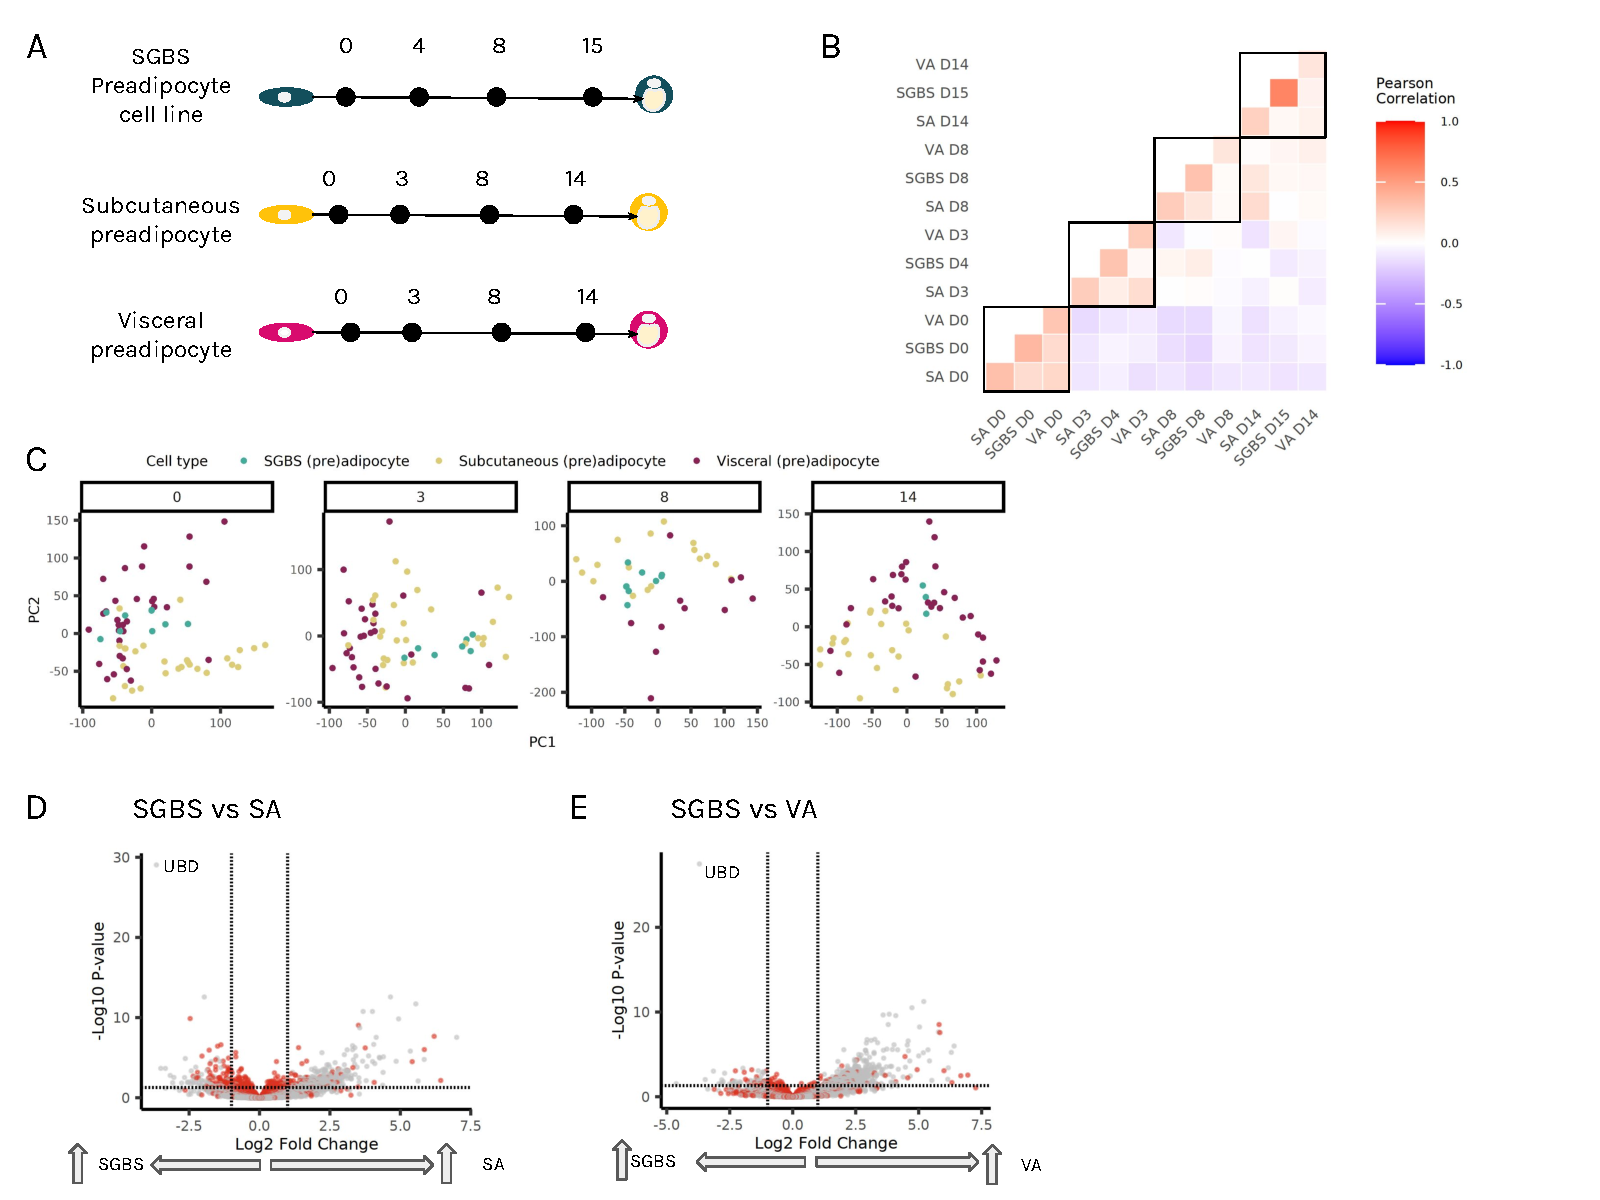
\includegraphics[width=\textwidth]{3_figures-and-files/Fig1.pdf}
    \caption[The transcriptional profiles of SGBS cells differ from both subcutaneous and visceral (pre)adipocytes.]{\textbf{The transcriptional profiles of SGBS cells differ from both subcutaneous and visceral (pre)adipocytes.} A. RNA-seq from 4 timepoints of differentiation was obtained for SGBS, subcutaneous, and visceral (pre)adipocytes. B. Pearson correlation applied on the PCs of each sample found more similarity by timepoint (black boxes) than the original source (VA, SA, SGBS). 
    C. PC 1 by PC 2 performed for each differentiation timepoint. For simplicity, days 3 and 4 were grouped together, and days 14 and 15 were put together. The SGBS cells, in teal, are found between the (pre)adipocytes of subcutaneous (yellow) and visceral (magenta) origin. 
    D, E. Volcano plots of the differential expression analysis performed for each depot against SGBS with the linear mixed model, $\mathrm{y} \sim \mathrm{depot} + (1 | \mathrm{timepoint})$. The red dots indicate genes with average expression of $>$ 1 CPM across all samples.
    }\label{fig: SGBS, subcutaneous, and visceral (pre)adipocyte transcriptional profiles}
\end{figure}

\subsection{Predicting transcription factors (TFs) to distinguish between subcutaneous and visceral (pre)adipocytes}

There are many existing methods to determine the TFs that define a cell type, ranging from purely computational to data-driven and validated\cite{Xu2021-bn,Joung2023-ft,Ng2021-kl,Ieda2010-rc,Stone2019-oe,Treutlein2016-hs}. Unfortunately, not all the databases include adipocytes or distinguish between types of adipocytes. Moreover, the methods that do have limited input samples for comparison between visceral and subcutaneous (pre)adipocytes. Thus, we applied the relevant ones to our question, and we complemented the results with our own analysis with a larger cohort of data.   

Mogrify predicts TFs for cell conversion by identifying those that are not only differentially expressed but also exert strong regulatory influence on other DEGs within a network\cite{Rackham2016-ef}. We ran the model to predict TFs to reprogram (pre)adipocytes between subcutaneous and visceral origins (\textbf{Figure 3.2A}). Intriguingly, the predicted TFs for the preadipocytes are not the same for the adipocytes. Moreover, KLF4 is both in the set for SPA to VPA and for VA to SA. The limited sample number (n=3 per celltype) from the FANTOM5 database is a caveat to these predictions.   

Another existing reference was built by D'Alessio and colleagues, which identifies candidate TFs using the Human Body Index collection\cite{D-Alessio2015-ia}. This algorithm evaluates the expression of each TF in the cell type of interest against the background of other cell types to determine candidate core TFs with high specificity to the cell type of interest. In this case, subcutaneous and visceral adipocytes are not being directly compared, but the TFs should reprogram a stem cell or fibroblast to SA or VA (\textbf{Figure 3.2A}). There are three redundant factors for the two cell types, PPARG, EBF1, and ZNF117, which would suggest that these three TFs are common for all adipocytes. While PPARG and CEBPA are required for differentiation from preadipocytes to adipocytes\cite{Lefterova2008-rk}, CEBPA is presented as a TF to reprogram a stem cell to a visceral adipocyte, which contradicts the Mogrify prediction that it would convert VA to SA. Collectively, Mogrify and D'Alessio models yield 46 TFs for depot-specific (pre)adipocyte reprogramming, accounting for overlaps and discrepancies between the models.

To further investigate these factors, we leveraged two independent cohorts of data from human subcutaneous and visceral (pre)adipocytes across differentiation\cite{Laber2023-qe,Bradford2019-ps}. Differential analysis was performed per timepoint and across four timepoints with a linear mixed model. Gene enrichment analysis and motif enrichment were applied to the DEGs to identify TFs that distinguish between the two depots. 38 of the 46 TFs are represented in the GSEA C3 Transcription Factor Targets Gene Set\cite{Liberzon2015-uo}, the HOMER human promoter set from RefSeq\cite{Heinz2010-lw}, and JASPAR2020\cite{Fornes2020-uo} (\textbf{Figure 3.2B}). The remaining 8 proposed TFs, DMRT2, ZNF117, PRICKLE1, SIK1, TXNIP, ARNTL2, IGF1, TSHZ2, should be tested experimentally.

\clearpage
\begin{figure}[!t]
    \centering
    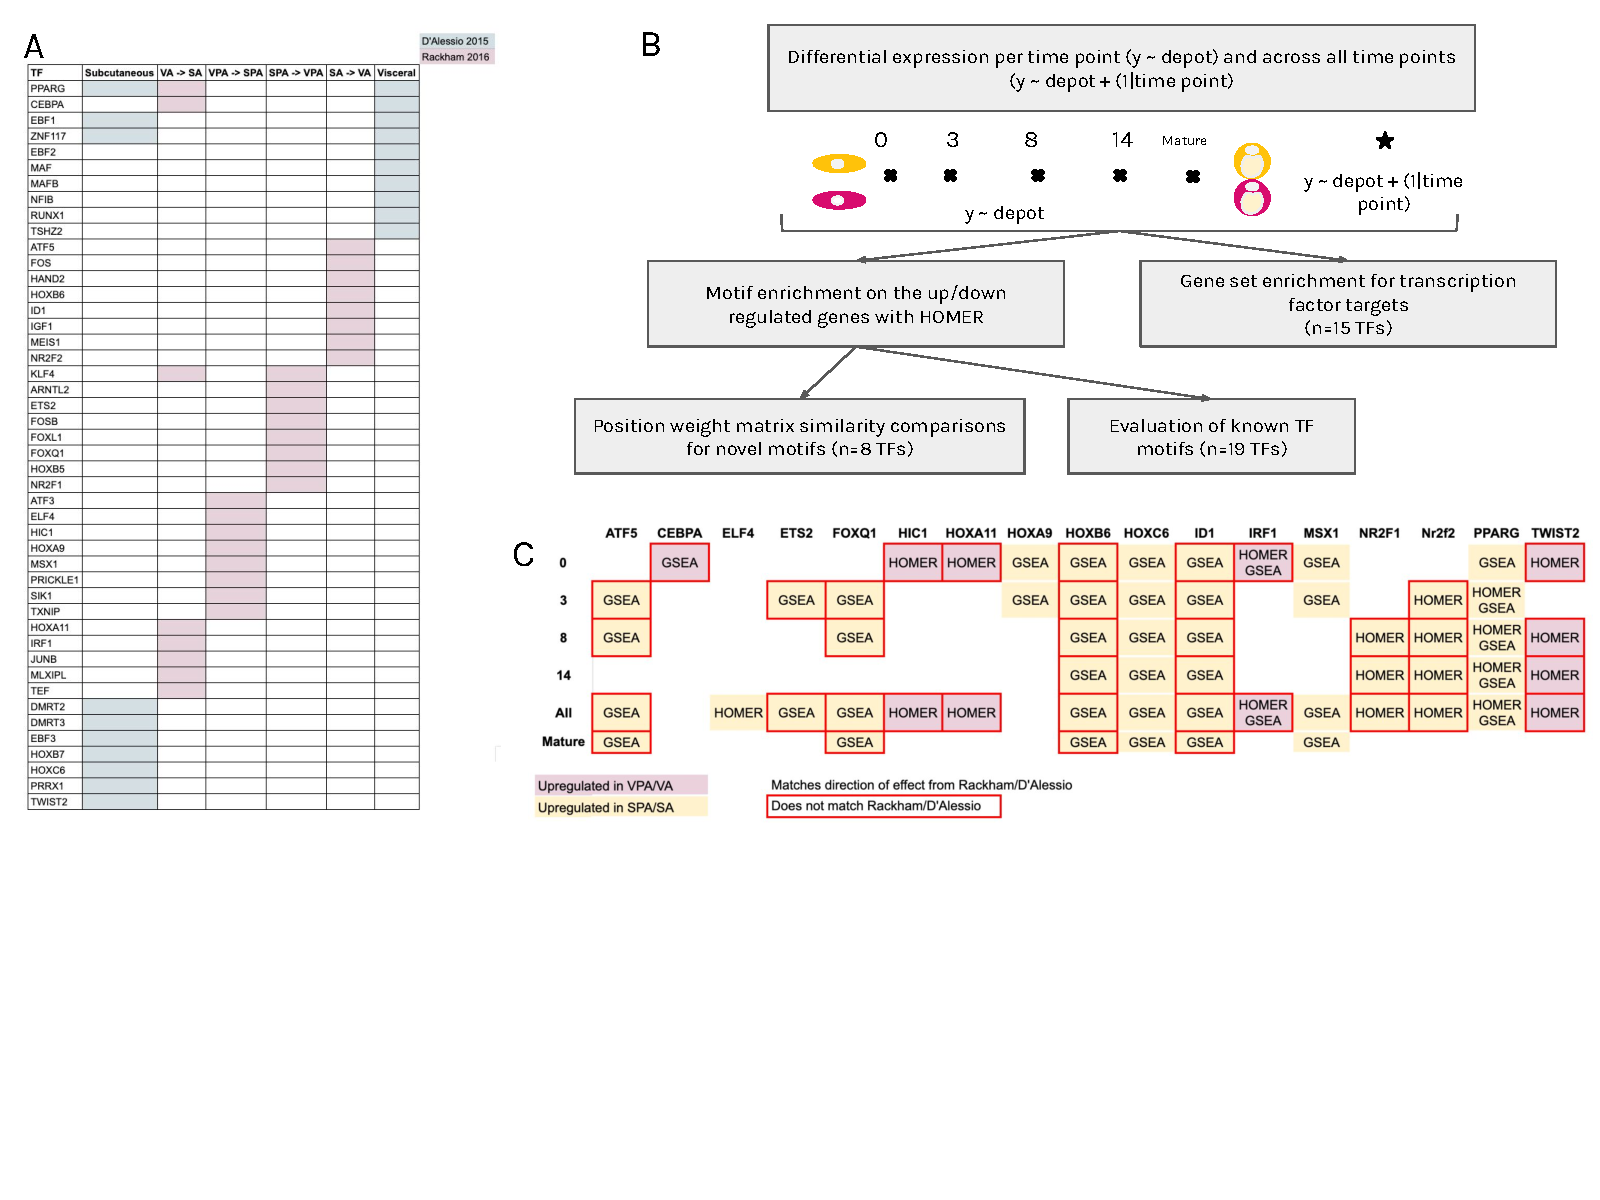
\includegraphics[width=\textwidth]{3_figures-and-files/Fig2.pdf}
    \caption[Candidate TFs predicted to distinguish between subcutaneous and visceral (pre)adipocytes include PPARG as a factor that is upregulated in subcutaneous (pre)adipocytes.]{\textbf{Candidate TFs predicted to distinguish between subcutaneous and visceral (pre)adipocytes include PPARG as a factor that is upregulated in subcutaneous (pre)adipocytes.} 
    A. The 46 TFs that are predicted to reprogram (pre)adipocytes from established methods. The colors indicate the data source. B. Workflow to evaluate the predicted TFs in two independent datasets\cite{Laber2023-qe,Bradford2019-ps}. Differential expression was performed for each timepoint and across all timepoints, and the results were put through motif enrichment and gene set enrichment analysis. C. Summary of the results from HOMER and GSEA, organized by differential expression model timepoint (row) and TF (column), colored by upregulation in subcutaneous (pre)adipocytes (yellow) or visceral (pre)adipocytes (pink). 5 TFs replicated in the same direction of effect, while 12 TFs were found in the opposite direction than predicted in A (red outline). 
    }\label{fig: Candidate TFs for depot specific reprogramming}
\end{figure}

17 of the predicted TFs were significantly enriched for either depot in at least one differential expression model across the TF identification methods (\textbf{Figure 3.2C}). The directional activity of each TF was internally consistent across the six models, with motif and gene set enrichment analyses identifying the same upregulated depot in every instance of overlapping detection. With the exception of ELF4, all the other TFs had significantly enriched activity in more than one model. Only 5 of these were concordant with the directionalities of the candidate reprogramming factors: ELF4, HOXA9, HOXC6, MSX1, and PPARG. PPARG was consistently enriched for subcutaneous (pre)adipocytes across five models and both gene set and motif enrichment analyses. 

D'Alessio predicted CEBPA as a factor for VA, which is supported by upregulated CEBPA activity in Day 0 visceral preadipocytes, but Mogrify identified CEBPA as a TF to convert VA to SA. HIC1, HOXA11, IRF1, and TWIST2 were predicted to identify subcutaneous (pre)adipocytes, but they are upregulated in visceral (pre)adipocytes. On the other hand, ATF5, ETS2, FOXQ1, HOXB6, ID1, NR2F1, and NR2F2 are all more active in subcutaneous (pre)adipocytes, despite initial predictions for visceral (pre)adipocyte fate. While gene expression does not necessarily correlate with transcription factor activity level\cite{Cheng2007-mc}, NR2F1 is more highly expressed in human visceral adipocytes\cite{Gesta2006-so}, which supports the Mogrify prediction. RUNX1 was nominally more active in visceral Day 3 preadipocytes than subcutaneous (p=0.01; q=0.0646), which is the predicted direction of effect from D'Alessio, but it was not found to be significantly enriched in visceral (pre)adipocytes. Overall, the minimal reproducibility of the TFs across the various methods highlights the need for more data. These results can be used to prioritize factors for testing, but all 46 proposed TFs should be evaluated for reprogramming.

\subsection{Developing a method to evaluate the reprogrammed cells}

After modification of SGBS cells with the proposed TFs, a robust analytical protocol is required to evaluate the reprogrammed state. To quantify reprogramming success, the transcriptomes of reprogrammed and thus unknown “query” cells will be captured via snRNA-seq and systematically benchmarked against reference profiles of both the original SGBS and target SA/VA cell types. We tested an assortment of computational conditions, including varying feature selection and integration methods, using two recent adipocyte snRNA datasets\cite{Emont2022-pb,Lazarescu2025-ru}. One limitation of sc/snRNA-seq is sparse data, in that there are many genes with zero counts, which can be biological, technical, or sampling in origin\cite{Jiang2022-yf}. To circumvent the sparse data and increase the reliability of results, pseudobulks can be generated for sc/snRNA-seq\cite{Squair2021-wz}. A pseudobulk is an aggregated transcriptional profile from a group of cells with the same label or cell type. It increases the stability of methods applied to sc/snRNA-seq data, such as differential expression or cell type classification\cite{Squair2021-wz,Adamson2016-gi}.   

\clearpage
\begin{figure}[!t]
    \centering
    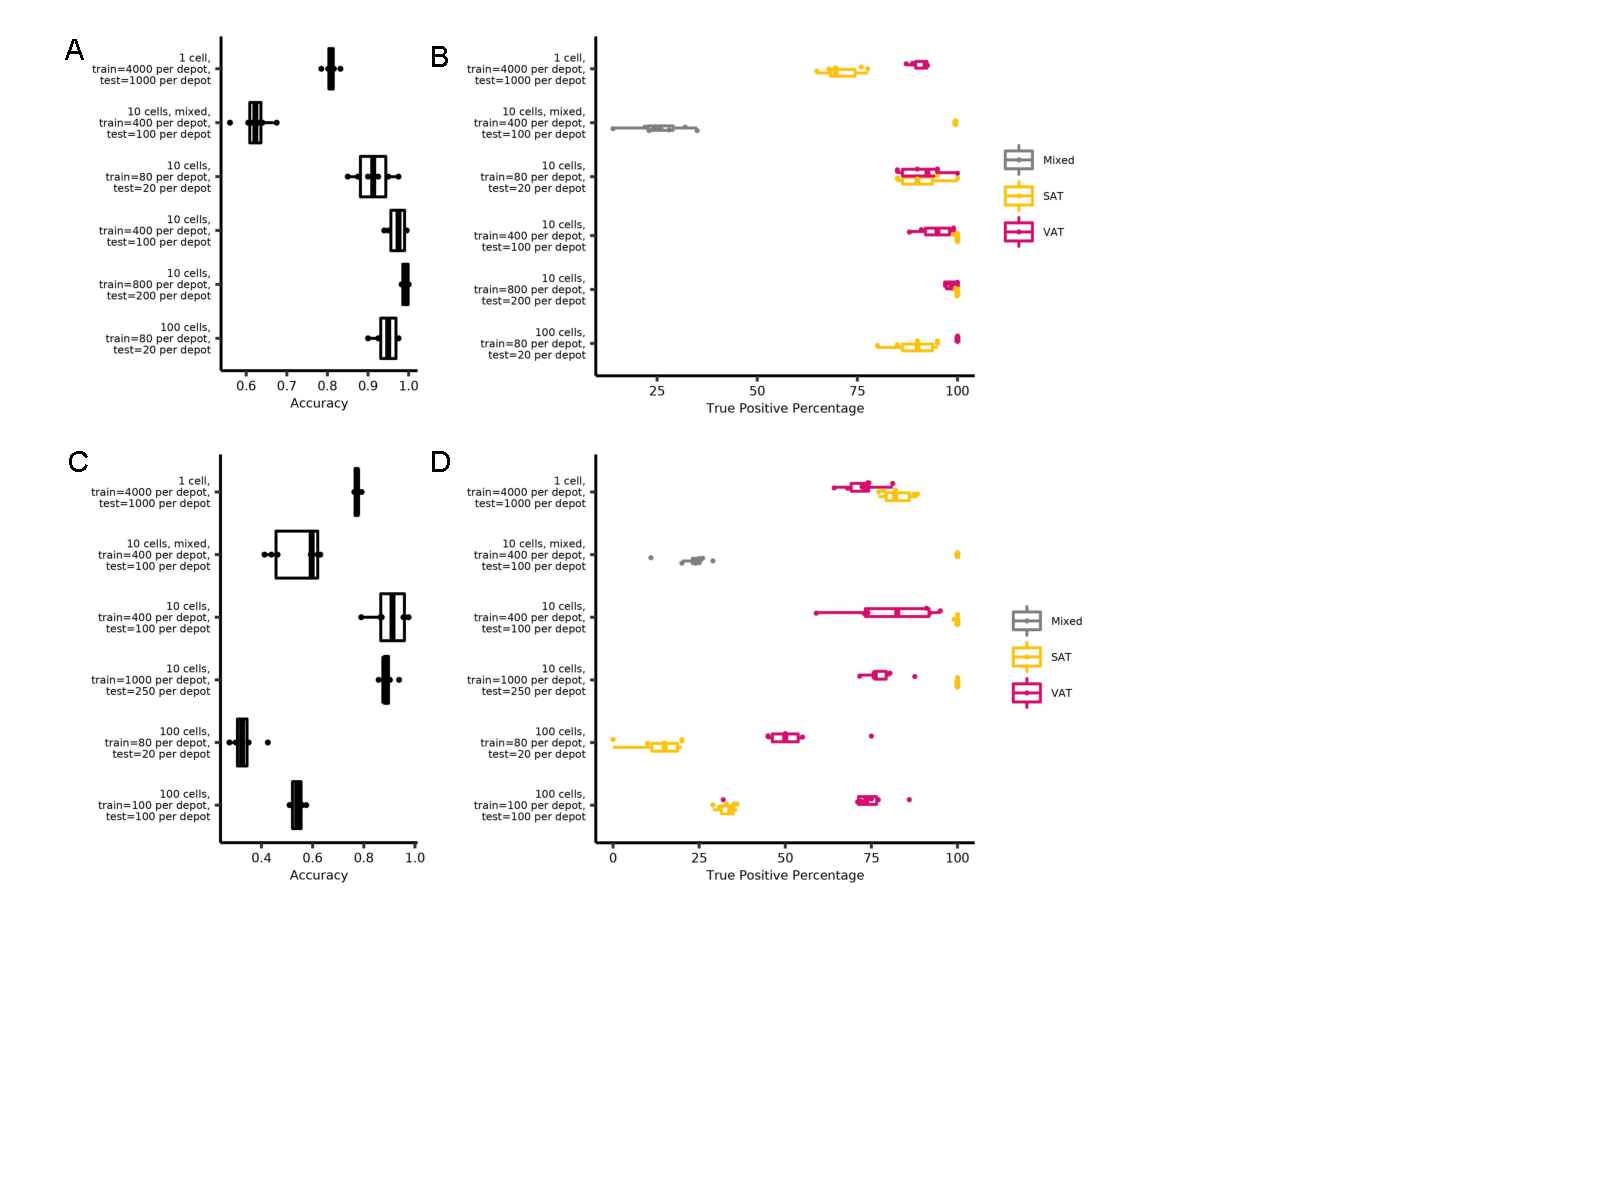
\includegraphics[width=\textwidth]{3_figures-and-files/Fig3.pdf}
    \caption[Pseudobulks of 10-cells with large training sets have high accuracy for predicting cell identity between subcutaneous and visceral adipocytes.]{\textbf{Pseudobulks of 10-cells with large training sets have high accuracy for predicting cell identity between subcutaneous and visceral adipocytes.} 
    A. Accuracy of Capybara models on Emont adipocytes. B. Percent of true positive results in the Emont models, separated by cell identity. C. Accuracy of Capybara models, trained on Emont data, tested on Lazarescu adipocytes. D. Percent of true positive results in the Lazarescu models, separated by cell identity. 
    }\label{fig: Evaluating cell identify with single cell RNAseq and pseudobulking}
\end{figure}

Capybara is an unsupervised computational method that scores cells against references using quadratic programming and has the framework to allow for multiple identities, including “multi” and “unknown”, enabling the identification of hybrid cells during reprogramming\cite{Kong2022-pg}. Capybara was run on the human adipocyte samples from Emont et al., using the single-cell data , pseudobulks generated from groups of 10 cells, and pseudobulks of 100 cells. A mixed population containing both visceral and subcutaneous adipocytes was also generated for the 10-cell pseudobulks to assess the multiple identity capacity within Capybara. With the single-cell data, the depot was correctly assigned with accuracy of 0.809$\pm$0.016, and the accuracy increased with pseudobulks (\textbf{Figure 3.3A}). Within the 10-cell pseudobulk, accuracy correlated with sample depth, from 0.972+0.023 with 500 pseudobulks per depot to 0.992+0.008 with 1,000 samples per depot. At the same sample depth of 100 samples, the 100-cell pseudobulks model (0.946+0.029) had higher accuracy than the 10-cell pseudobulk model (0.876+0.039). This indicates that the accuracy and precision of the predictions could be even greater with more samples. The results are bolstered by the mixed depot 10-cell pseudobulks, which had the lowest accuracy (0.633+0.024) and faithfully identified that there were mixed samples, detecting 25.5\% of the mixed pseudobulks (\textbf{Figure 3.3B}). Unexpectedly, the true positive rates of each depot varied between conditions. Subcutaneous adipocytes had a lower true positive percentage (70.9$\pm$1.99) in the single-cell and 100-cell pseudobulk models compared to visceral adipocytes (90.8$\pm$0.918), while the opposite trend held for most of the 10-cell pseudobulks (\textbf{Figure 3.3B}). This could be attributed to missing or lowly expressed genes that contribute significantly to cell identity. 

To increase sample number and test how the models work across datasets, the Emont-integrated transcriptomes from the Lazarescu et al. adipocytes were pseudobulked and classified (\textbf{Figure 3.3C, D}). The 10-cell pseudobulk model outperformed both the single-cell and 100-cell approaches, achieving accuracies of 0.903$\pm$0.073 and 0.890$\pm$0.027 across two sample depths. In comparison, the single-cell model reached an accuracy of 0.774$\pm$0.011, and the 100-cell pseudobulk 0.333$\pm$0.0517, at the same split ratio. While increasing the sample depth with an adjusted split ratio improved the 100-cell model, its accuracy remained low (0.540$\pm$0.0251) due to insufficient input data. Both 100-cell models were surpassed by the depot 10-cell pseudobulk model in accuracy (0.547$\pm$0.092), further indicating that more samples are necessary when combining different sc/snRNA datasets, even with computational integration. Intriguingly, the true positive percentage for subcutaneous adipocytes still approached 100\% in the 10-cell pseudobulk methods, and the predictions for visceral adipocytes were less accurate. This suggests that the transcriptional signature of subcutaneous adipocytes is more robust than visceral adipocytes. Altogether, despite being trained and tested on different datasets, the 10-cell pseudobulk models predicted cell identity with $>$0.890 accuracy, which is highly promising for future applications.

\section{Discussion}

In this chapter, we set up the analytical framework for reprogramming depot-specific adipocytes. We explored whether SGBS cells would be suitable progenitors to model human (pre)adipocytes from both subcutaneous or visceral origin through transcriptomics. The TFs to convert precursors to SA and VA were evaluated using a series of curated methods, and models scoring the success of reprogramming were explored. This novel proposal is unique in its application of cell identity methods and pseudobulking on depot-specific adipocytes.   

The 46 candidate TFs we identified for subcutaneous and visceral (pre)adipocyte reprogramming are well supported in the literature. In this chapter, PPARG was consistently found across many time points and modalities as having upregulated activity in subcutaneous (pre)adipocytes. This aligns with previous data for mouse and human adipocytes: in human preadipocyte samples, visceral adipocytes have lower expression of adipogenic factors, including PPARG\cite{Mathur2022-fx}; in mouse cells, visceral preadipocytes cultured ex vivo require BMP-4 in addition to the standard differentiation cocktail to induce expression of Pparg and stimulate adipogenesis\cite{Macotela2012-wy}; and human SA have reduced methylation at \textit{PPARG} and its binding partner RXRa compared to VA\cite{Bradford2019-ps}. Moreover, familial partial lipodystrophy type 3 (FPLD3) is caused by pathogenic variants in PPARG\cite{Rutkowska2022-rs}. This rare genetic disorder results in a loss of subcutaneous fat from lower limbs without affecting visceral fat accumulation, highlighting the depot-specific activity of PPARG.

Additionally, 6 HOX TFs were predicted to induce depot-specificity, and the literature contains many examples of differentially expressed HOX genes between depots, although not all of our predictions are concordant with existing knowledge\cite{Ahn2019-us,Gesta2007-cp}. One that is consistent is HOXA9, which is more active in subcutaneous (pre)adipocytes and has been observed to be more highly expressed in SAT than VAT\cite{Tchkonia2007-xa}.  

Furthermore, a genome wide methylation study performed on SA and VA examined TF binding motifs within 150 base pairs of the methylated sites and identified 49 transcription factors that corresponded to 7 binding motifs in SA\cite{McAllan2023-qo}. 9 of these overlapped with our 46 of interest, including 5 that were intended for reprogramming into SA: ATF3, JUNB, KLF4, ELF4, and HOXA11. Lazarescu et al. also identified TFs of interest for depot-specificity using SCENIC, a method for regulatory network and cell identity clustering\cite{Aibar2017-wj}. They found one regulon that is different between visceral and subcutaneous adipocytes, containing CEBPA, which was enriched in VA but not SA, as well as RUNX1. This is concordant with the D'Alessio predictions and the gene set enrichment results. The genes enriched for subcutaneous adipocytes were STAT4 and RELA, which were not in our set of 46\cite{Lazarescu2025-ru}. In addition, lineage tracing studies have identified Prx1 as a selective marker for subcutaneous adipocytes and Wt1 for visceral preadipocytes\cite{Sakers2022-wb}. Collectively, these studies suggest a broader landscape of candidate TFs for (pre)adipocyte reprogramming.  

The significance of this work would include not only the computational methods but also the physical resource of depot-specific (pre)adipocytes to enable further research. Visceral adipocytes contribute to ovarian cancer metastasis\cite{Nieman2011-hq} and are associated with ovarian cancer chemoresistance\cite{Lin2024-ov}. The study that identified the chemoresistance correlation used a 3-cell coculture model, in which the adipocytes were either primary culture omental adipocytes or differentiated 3T3-L1 cells, which are a mouse preadipocyte cell line. The objective of this work would be to enable future investigators to use a human visceral adipocyte cell line instead of the mouse fibroblast. Furthermore, there was internal consistency in the TF predictions, but many of the candidate 46 were not uncovered by the enrichment analyses. This could be indicative of differences between initial data sources, especially with the caveats that the subcutaneous and visceral (pre)adipocyte transcriptomic data is derived from cells differentiated ex vivo\cite{Laber2023-qe}, while the Mogrify model had three replicates per cell type\cite{Rackham2016-ef}. This highlights the need to reprogram depot-specific adipocytes to enable future comparisons. The factors identified could be applied to cell types other than SGBS cells, such as stem cells and induced pluripotent stem cells, such that the effects of genetic mutations on visceral versus subcutaneous adipocytes could be robustly compared.  

While this framework provides a theoretical blueprint for depot-specific reprogramming, several limitations remain. The current reliance on transcriptomic data provides a high-resolution snapshot of cell state, but lacks the epigenetic context required to fully map the regulatory landscape. Future iterations of this model would benefit from the integration of ATACseq data to further refine the candidate set of 46 factors\cite{Halasz2023-xu,Lee2024-ix}. Furthermore, while our pseudobulking approach successfully prevented data leakage and ensured internal consistency, the resulting data bottleneck for the 100-cell models suggests that future studies utilize even larger datasets to improve model generalizability. Ultimately, the transition from this computational framework to in vitro experimental validation will be the definitive test of these predicted TFs. Several critical parameters remain to be optimized, including the number of TFs delivered simultaneously, the activation method (e.g., viral overexpression or CRISPRa), and the specific “dosage” of each factor. Because many identified TFs exhibit activity in both subcutaneous and visceral depots, achieving the precise threshold of upregulation necessary to drive a depot-specific identity is essential. Addressing these pending questions will move us closer to generating subcutaneous and visceral (pre)adipocyte cell lines.   

This work establishes a novel analytical framework for the depot-specific reprogramming of human adipocytes, utilizing SGBS cells as a versatile progenitor model. By integrating multiple transcriptomic datasets and literature-backed methods, we generated a candidate set of 46 transcription factors to identify key regulators of depot identity, such as PPARG and members of the HOX family. We further applied pseudobulking without replacement to a cell identification method to create high-fidelity models for scoring adipocyte reprogramming and demonstrated that 10-cell pseudobulks provide optimal predictive accuracy. This research provides a theoretical foundation for creating human subcutaneous and visceral (pre)adipocytes from the same original cell line, offering a more physiologically relevant alternative for studying adipocytes and adipocyte-driven pathologies.

%%%%%%%%%%%%%%%%%%%%%%%%%%%%%%%%%%%%%%%%%%%%%%%%%%%%%%%%%%%%%%%%%%%%%%%%%%%%%%%%
\section{Methods}
%%%%%%%%%%%%%%%%%%%%%%%%%%%%%%%%%%%%%%%%%%%%%%%%%%%%%%%%%%%%%%%%%%%%%%%%%%%%%%%%

\subsection{Analysis of bulk RNA-seq datasets}

We analyzed the bulk RNA-seq datasets of human derived subcutaneous and visceral adipocytes (GSE184089 and GSE110821) and SGBS cells (GSE274839, GSE245619, and GSE262480). Raw sequencing reads were aligned to the reference hg38 using Kallisto with default parameters\cite{Bray2016-zt} to generate gene counts per sample. Analysis was performed in R 4.1.3.   

In GSE184089, adipose derived mesenchymal stem cells (AMSCs) were sequenced at four timepoints of adipocyte differentiation, from early preadipocytes to full adipocytes. 2 outliers were removed, and 3 samples were relabeled after initial processing indicated they were mislabeled.

\subsubsection{Visualizing the transcriptional profiles of SGBS, subcutaneous, and visceral (pre)adipocytes}
ComBat-seq was run between datasets (GSE274839, GSE245619, GSE262480, and GSE184089) for batch correction\cite{Zhang2020-kq}. The smallest group was the Day 15 SGBS samples (n=3), and the largest were the visceral Day 0 preadipocytes and visceral Day 14 adipocytes (n=32). EdgeR 3.36.0 and limma-voom (limma v3.50.1) were used to filter and normalize reads for library size\cite{Robinson2010-qx,Law2014-yh}. 28,757 genes were retained across 234 samples. PCA was performed with prcomp() across all samples and by time point. The correlation plot was generated from the cor() on the PCA results of the full dataset, taking the average per cell type and time point. 

\subsubsection{Differential expression between SGBS, subcutaneous, and visceral (pre)adipocytes}
ComBat-seq was run between datasets (GSE274839 and GSE184089) for batch correction\cite{Zhang2020-kq}. EdgeR 3.36.0 and limma-voom (limma v3.50.1) were used to filter and normalize reads for library size\cite{Robinson2010-qx,Law2014-yh}, retaining 27,134 genes and 218 samples. Differential expression was performed for each depot (subcutaneous and visceral) against SGBS in dream\cite{Hoffman2021-xx} using a linear mixed model with gene expression as a result of fixed effect depot and random effect differentiation day, $\mathrm{y} \sim \mathrm{depot} + (1 | \mathrm{day})$.

\subsection{Identifying candidate transcription factors}
Mogrify and the atlas built by D'Alessio were used as directed by the manuscripts\cite{Rackham2016-ef,D-Alessio2015-ia}. For Mogrify, each TF is ranked based on a weighted sum of its regulatory influence, and the optimal set of TFs is selected to account for 98\% of regulatory coverage \cite{Rackham2016-ef}. Its database has n=3 for each SPA, VPA, SA, and VA.

\subsubsection{Differential expression between subcutaneous and visceral (pre)adipocytes}
EdgeR 3.36.0 and limma-voom (limma v3.50.1) were used on GSE184089 to filter and normalize reads for library size\cite{Robinson2010-qx,Law2014-yh}, retaining 24,269 genes and 206 samples. A cell-means linear model, in which samples were categorized into eight discrete groups representing each depot-time combination (SA and VA; Days 0, 3, 8, and 14), was performed in dream\cite{Hoffman2021-xx}, and contrasts were calculated between each depot for every time point. In addition, a linear mixed model with gene expression as a result of fixed effect depot and random effect differentiation day, $\mathrm{y} \sim \mathrm{depot} + (1 | \mathrm{day})$. For the mature adipocytes, edgeR 3.36.0 and limma-voom (limma v3.50.1) were used on GSE110821 to filter and normalize reads for library size, retaining 13,1472 genes and 6 samples, and perform differential expression analysis by depot\cite{Robinson2010-qx,Law2014-yh}.

\subsubsection{TF identification}
TF Gene set enrichment was run with fgsea v1.20.0\cite{Korotkevich2021-ra} on the transcription factor pathways in Gene Ontology C3 transcription factor targets (TFT) using the parameters minSize=10, maxSize \= 1500, and nPermSimple=10000\cite{Subramanian2005-bj,Mootha2003-ys}. FindMotifs was run in HOMER with the parameters \-start \-1000 \-end 1000\. 8 TFs have known motifs in JASPAR but are not present in either the GO C3 TFT collection or the HOMER Refseq promoter set. These genes are PRRX1, DMRT3, EBF3, FOSB, HOXB5, NFIB, MLXIPL, and FOXL1. To determine if any of these TFs were enriched, the position weight matrices (PWMs) for these transcription factors were scored against the top novel HOMER results. There were no Pearson correlations greater than 0.7, indicating that none of the novel motifs align with the motifs of these 8 TFs.  

\subsubsection{Processing adipocyte sc/snRNA-seq}
Human adipocyte snRNA-seq was downloaded in rds format from the Emont lab\cite{Emont2022-pb}. Analysis was performed in R 4.3.1 with Seurat 4.3.0.1. The adipocytes were subset into two objects by depot (11,475 visceral adipocytes and 14,396 subcutaneous adipocytes), and a sparse matrix of the raw counts from each object was exported. Pseudobulks without replacement were generated in 10 and 100-cell iterations. Mixed 10-cell pseudobulks were created with commonly expressed genes and equal proportions of VA and SA cells (n=2,294).  

The snRNA-seq of human subcutaneous and visceral adipocytes, integrated with Emont et al., were downloaded from CZ CELLxGENE\cite{Lazarescu2025-ru,CZI-Cell-Science-Program2025-eh}. Analysis was performed in R 4.3.1 with Seurat 4.3.0.1 after the h5ad file was converted into a Seurat Object. There were 26,601 subcutaneous adipocytes and 26,935 visceral adipocytes. Pseudobulks were generated as described above. 

\subsection{Implementing Capybara}
The cell identification method was applied following the original protocol \newline https://github.com/morris-lab/Capybara with a few modifications\cite{Kong2022-pg}. For each iteration, the snRNA sparse matrices were randomly subset and formatted to match the Capybara reference and test matrices. There were an equal number of SA and VA (or SA and mixed) samples for each test dataset and train dataset. A high-resolution reference was constructed from the reference matrix and metadata, and quadratic programming was performed on the reference and subsequently on the test. Cell types were then classified and scored. For each condition, n=6 for SA vs VA, and n=8 for SA vs mixed.

\subsection{Proposed experimental outline}
We will use CRISPR activation (CRISPRa) to overexpress our TFs of interest in SGBS cells. The advantages of this model over other forms of induced overexpression are the high multiplexing capacity and direct transcriptional activation from endogenous loci activation \cite{Sokka2022-ax}. There have been CRISPRa reprogramming screens \cite{Yang2019-wd,Liu2018-fc}, and targeted CRISPRa for the reprogramming of lymphoblastoid cell lines to induced pluripotent cells showed high fidelity and homogeneity, indicating it can be more successful than conventional methods \cite{Sokka2022-ax}.   

SGBS cells will be transduced with a doxycycline-inducible dCas9-VPR to generate a CRISPRa cell line. The 46 transcription factors identified will be activated singly and in pairwise combinations using CROPseq-multi\cite{Walton2024-xj}. A library of constructs consisting of single and dual guide RNAs (sgRNAs) corresponding to each of the TFs, with two independent sgRNAs per TF, and 20\% non-targeting control (NTC) sgRNAs, will be constructed. The sgRNAs will be identified through CRISPick, which optimizes differently for CRISPRa/i guides\cite{Sanson2018-bh,Doench2016-bp}. Chromosomal positioning of the sgRNAs will also be taken into account to optimize the binding of many activators to the promoter region.   

This library will be transduced at MOI=0.15 into the dCas9-VPR inducible SGBS adipocytes such that each perturbation is replicated in 1000 cells. After 7 days, the transduced SGBS cells will be subjected to scRNA-seq using the 10x Genomics platform as detailed in the preliminary data to generate a per cell transcriptomic profile. Notably, the sgRNA vector design enables for each cell identification of the sgRNAs transduced as well activation of the target TF. Thus only cells with successfully induced activation will be retained for analysis\cite{Walton2024-xj}.   

As alternatives, we will also explore transgenes and multiplexed open reading frames, in case the CRISPRa SGBS cell line is not viable\cite{Joung2023-ft}.

% References
\bibliographystyle{unsrtnat}
\bibliography{bib_3.bib}